\section{Results}
\label{sec:results}
\subsection{Purity}
Here we present once again the final purity results to make clear what we will include in the paper on this analysis.

\begin{figure}[h]
\center
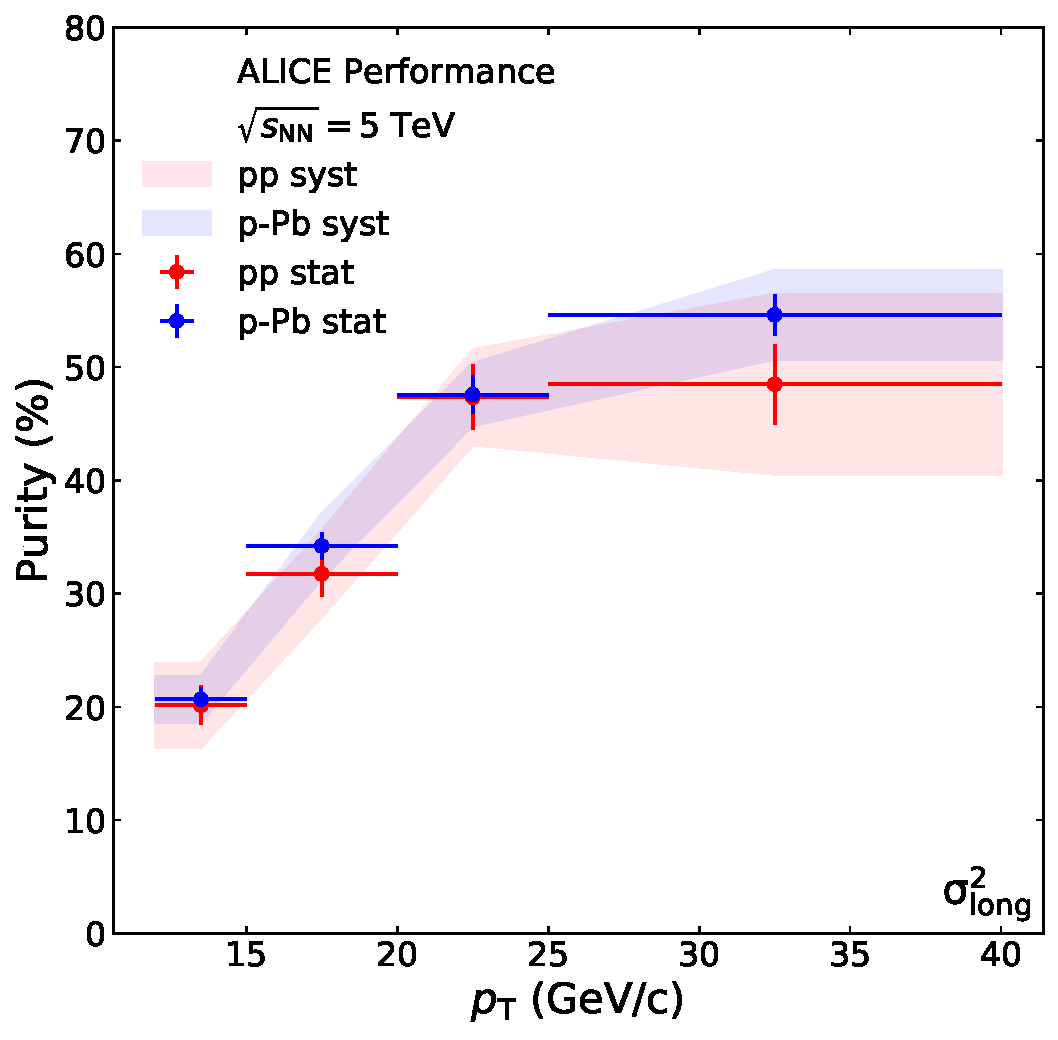
\includegraphics[width=0.495\textwidth]{Purity/purities-combined-cluster_Lambda.pdf}
\caption{Purity of isolated-photon selection as a function of cluster \pt. The error bar represents statistical uncertainty only. The error band represents the systematic uncertainty only.}
\label{fig:purityresults_again}
\end{figure}


Figure \ref{fig:purityresults_again} shows the final purities in pp and \pPb as a function of cluster \pt. This figure is identical to Figure \ref{fig:purityresults}.



\subsection{Azimuthal correlations in pp and \pPb~data}


Figure~\ref{fig:CorrelationFinal} shows the fully-corrected $\gammaiso$--hadron correlations in pp and~\pPb. The band at zero represents the uncertainty from the uncorrelated background estimate. The vertical error bars represent the statistical error bars only. We observe an agreement within uncertainties between pp, \pPb, and \textsc{PYTHIA 8.2} Monash tune in the presented $\zt$~range. We quantify this by means of a $\chi^{2}$ test between pp and \pPb~data that considers all uncertainties and their correlation among the different $\Delta\varphi$ bins. No significant difference is observed ($p$ values always larger than 0.05).   

\begin{sidewaysfigure}
\centering
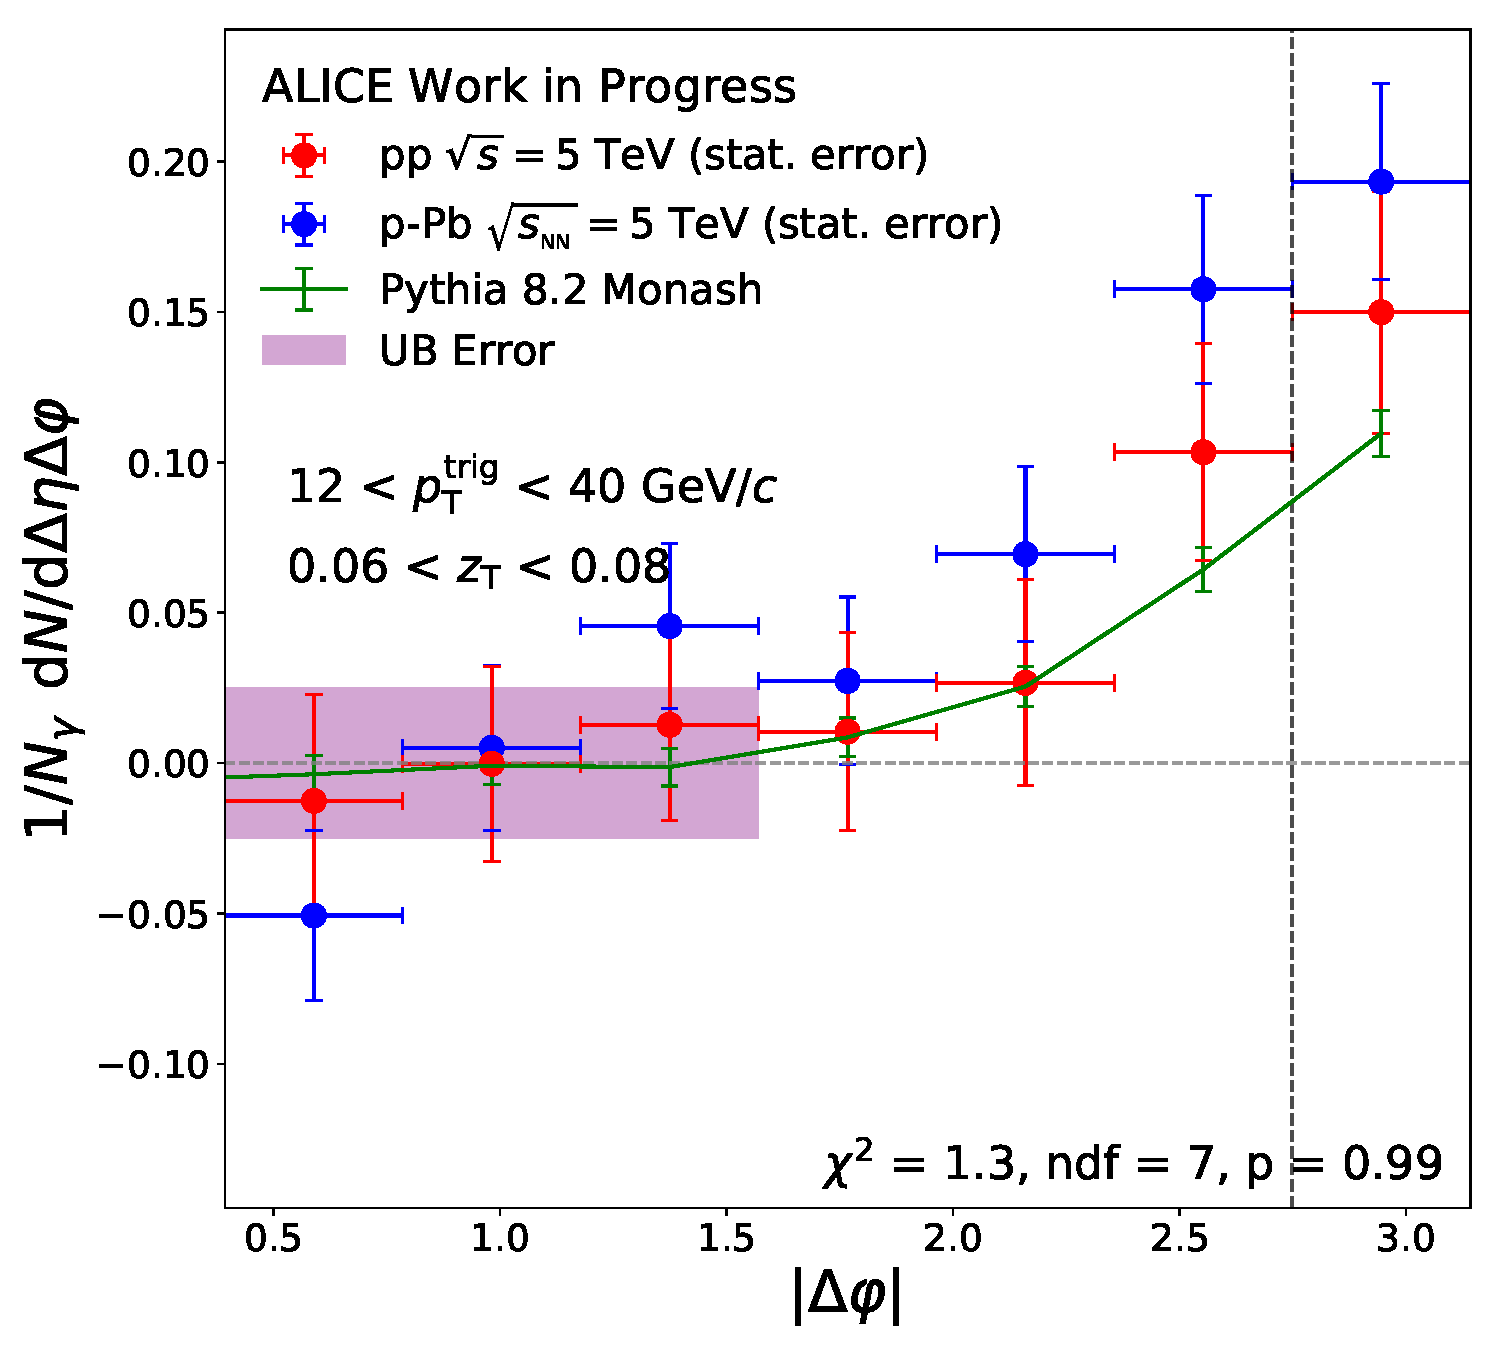
\includegraphics[width = 0.24 \textwidth]{G-H_New/Cs_Final_Indv_pT_0_zT_0.pdf}
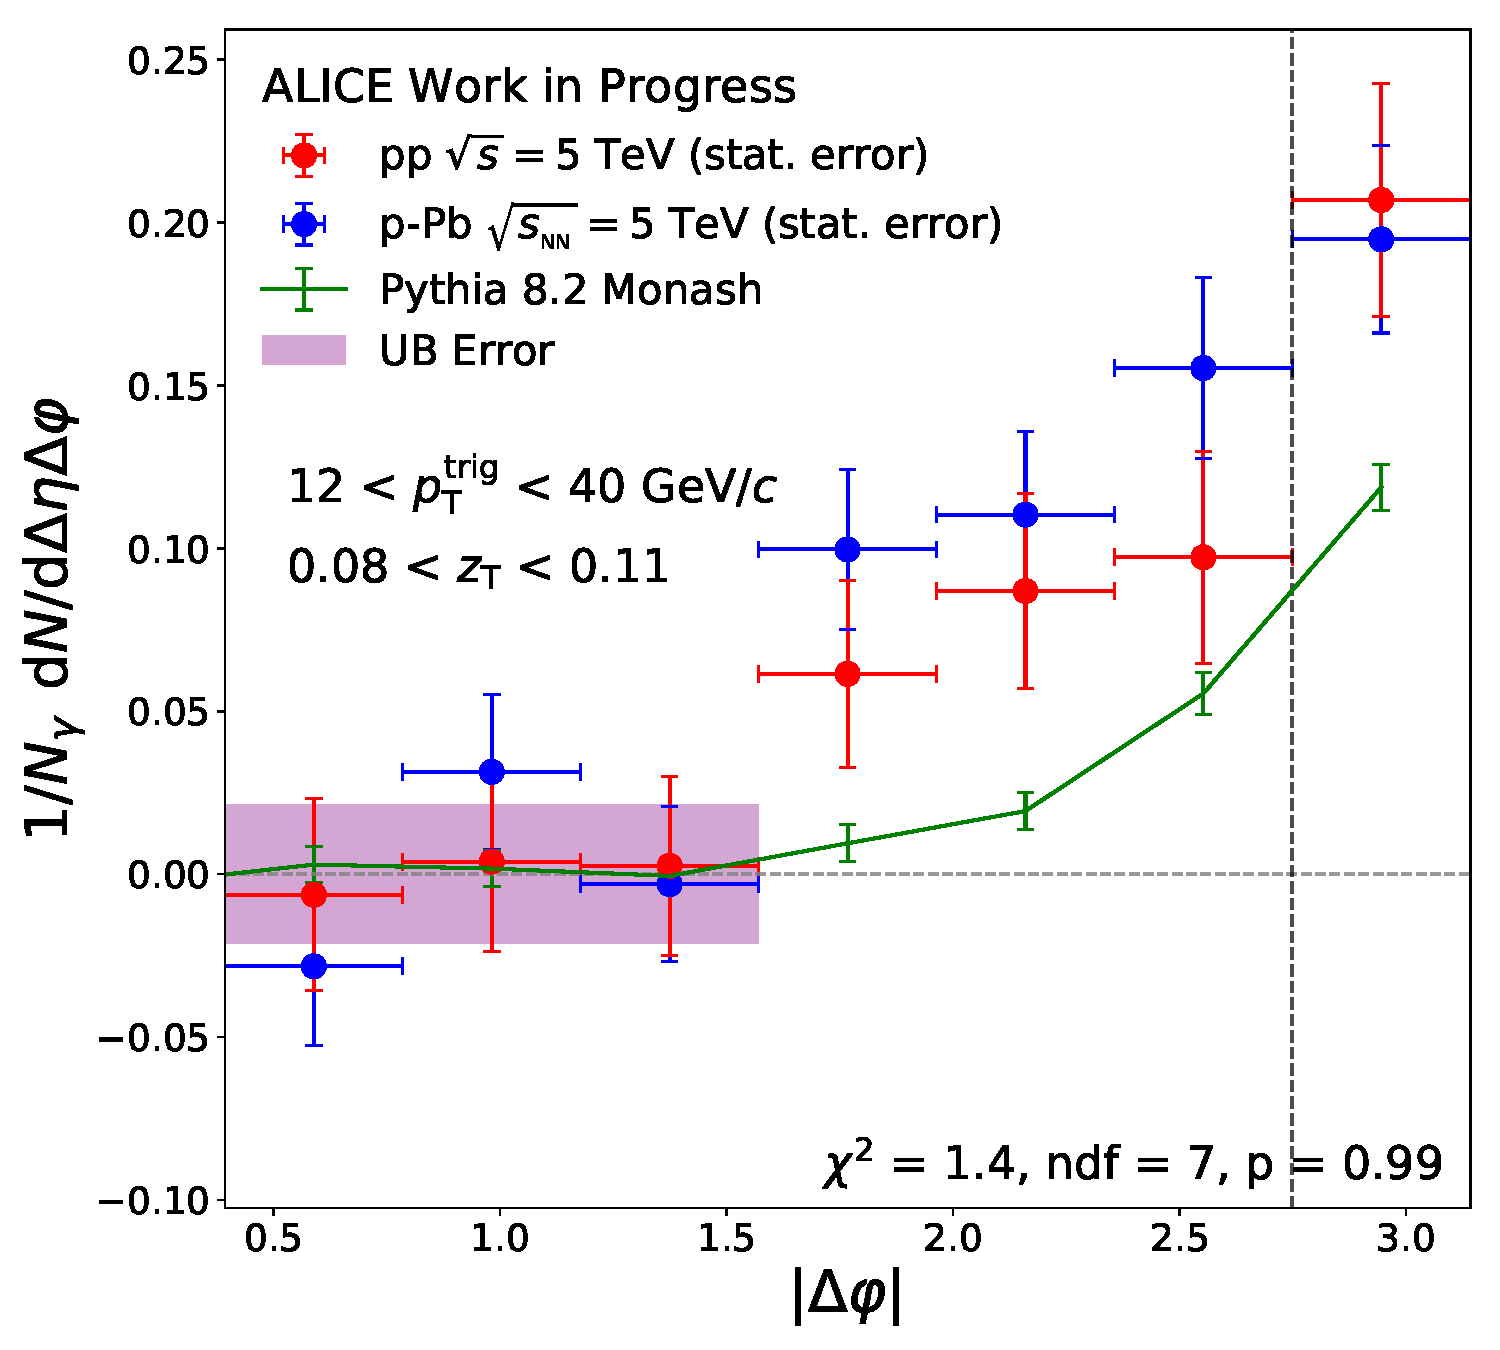
\includegraphics[width = 0.24 \textwidth]{G-H_New/Cs_Final_Indv_pT_0_zT_1.pdf}
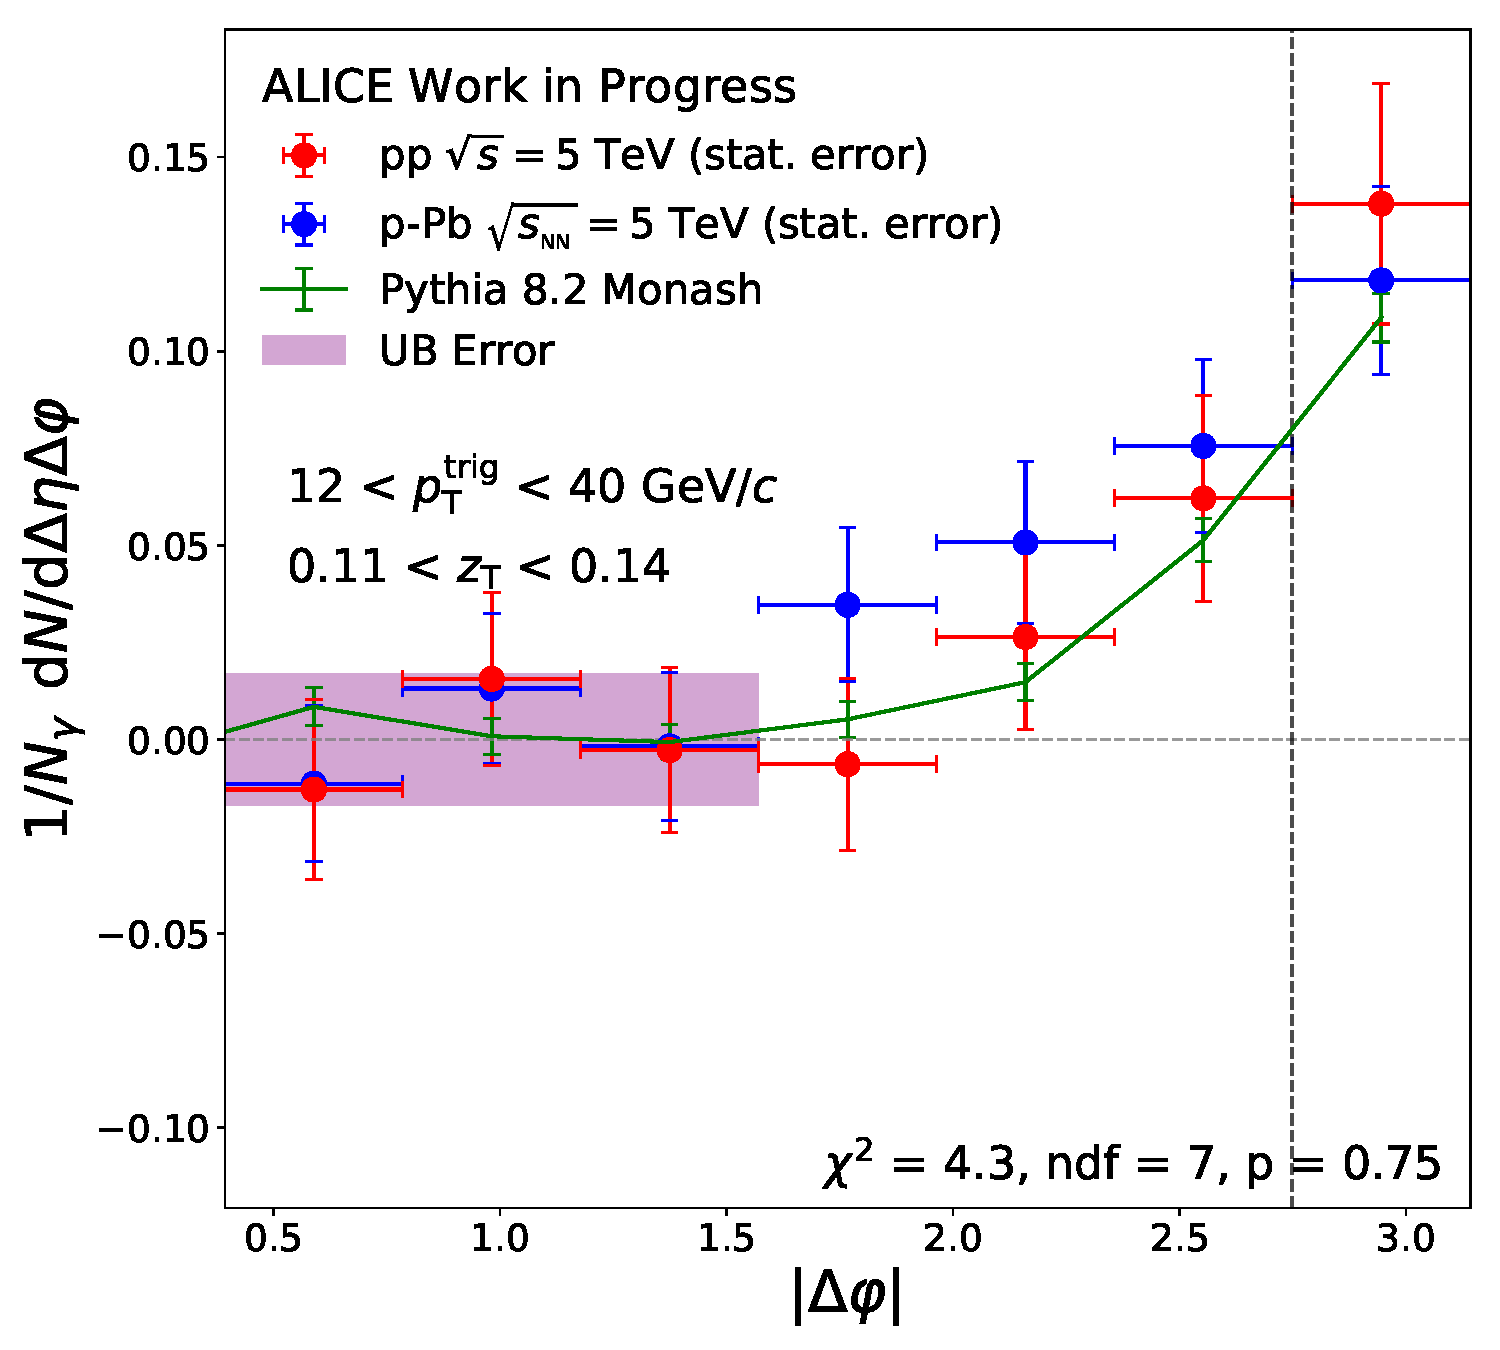
\includegraphics[width = 0.24 \textwidth]{G-H_New/Cs_Final_Indv_pT_0_zT_2.pdf}
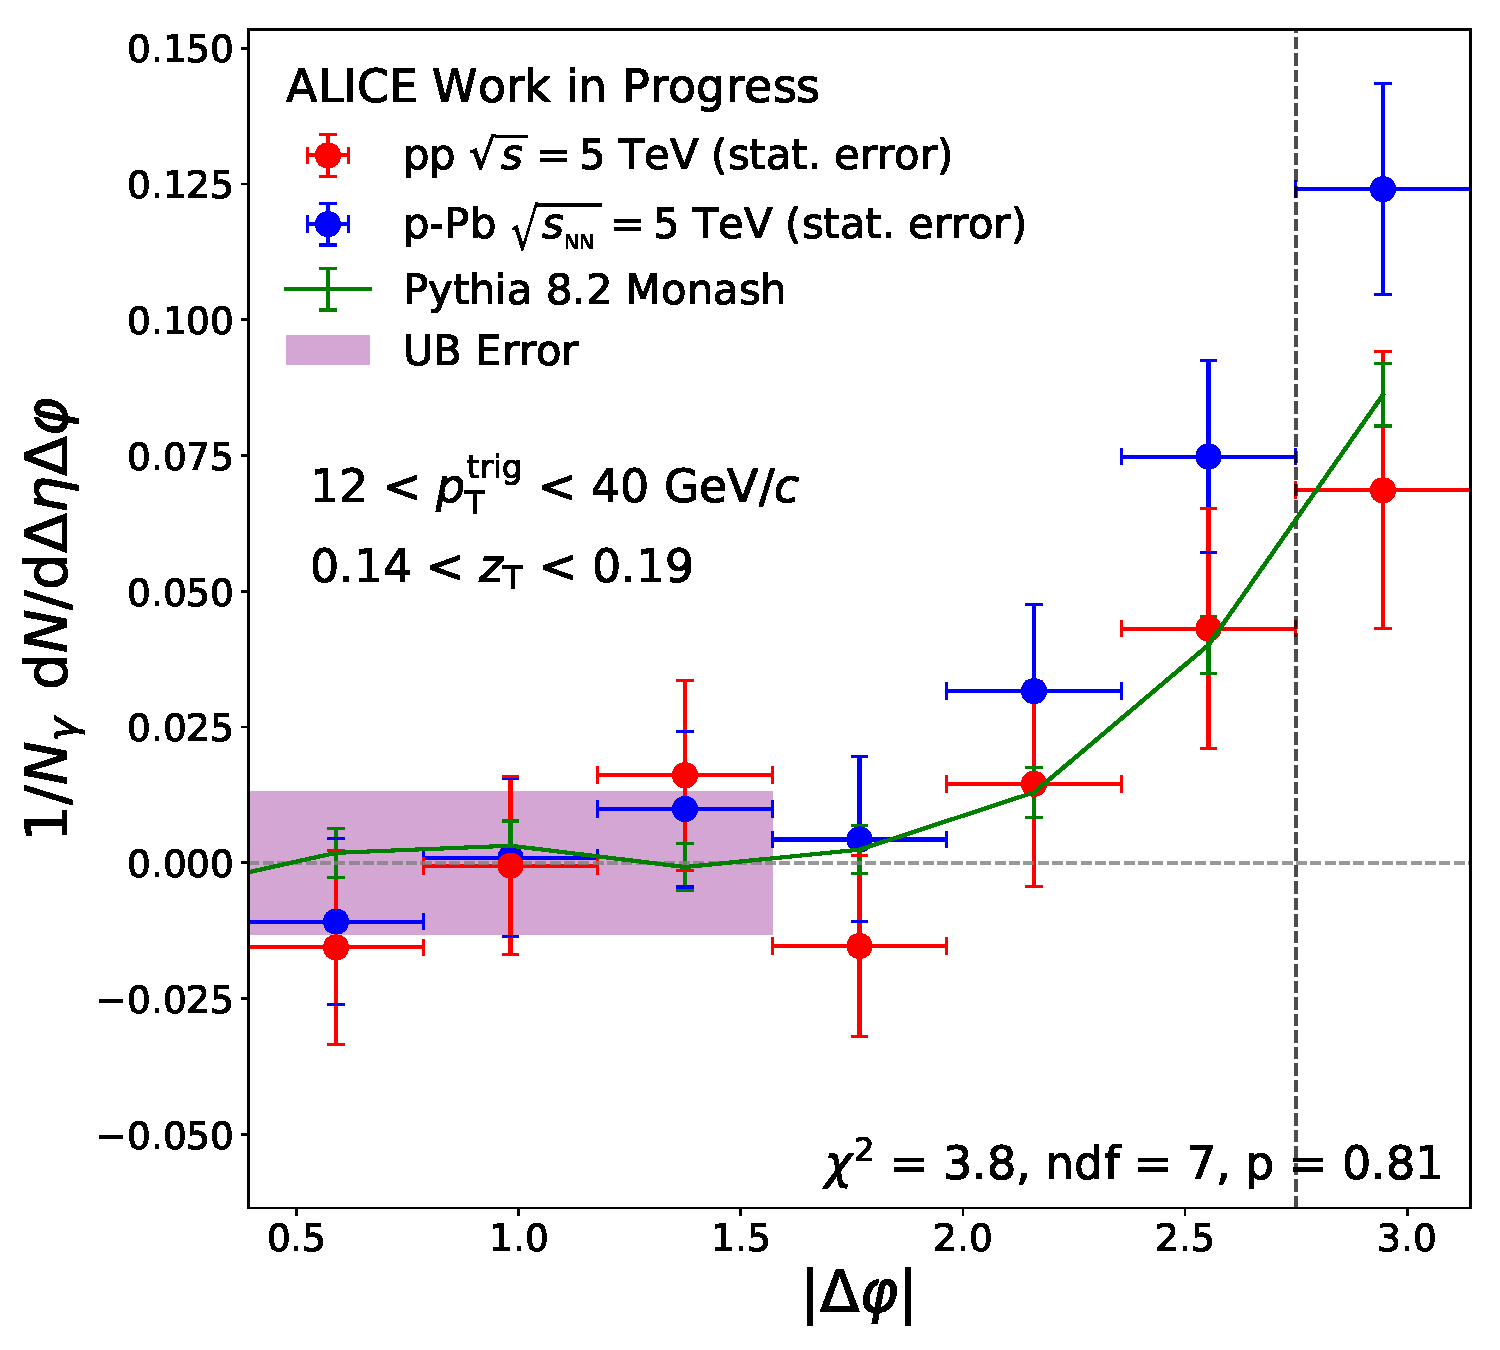
\includegraphics[width = 0.24 \textwidth]{G-H_New/Cs_Final_Indv_pT_0_zT_3.pdf}
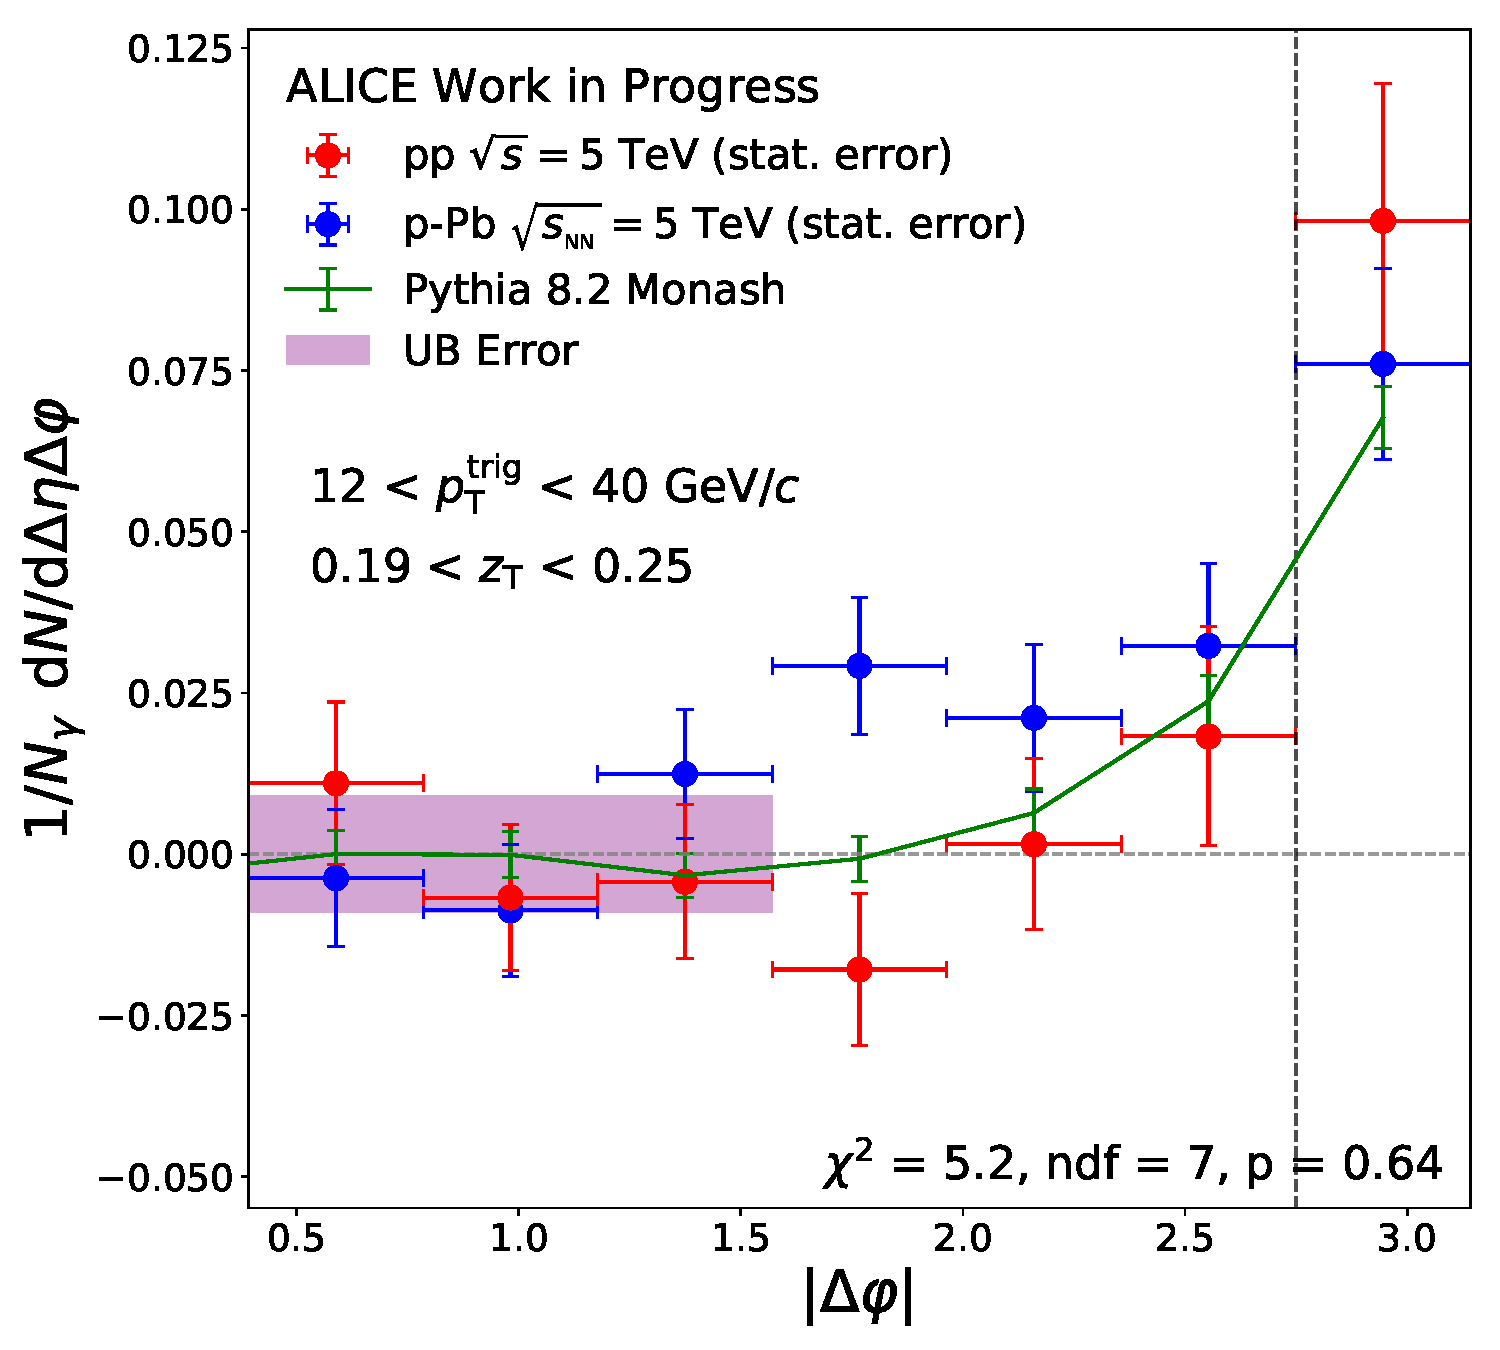
\includegraphics[width = 0.24 \textwidth]{G-H_New/Cs_Final_Indv_pT_0_zT_4.pdf}
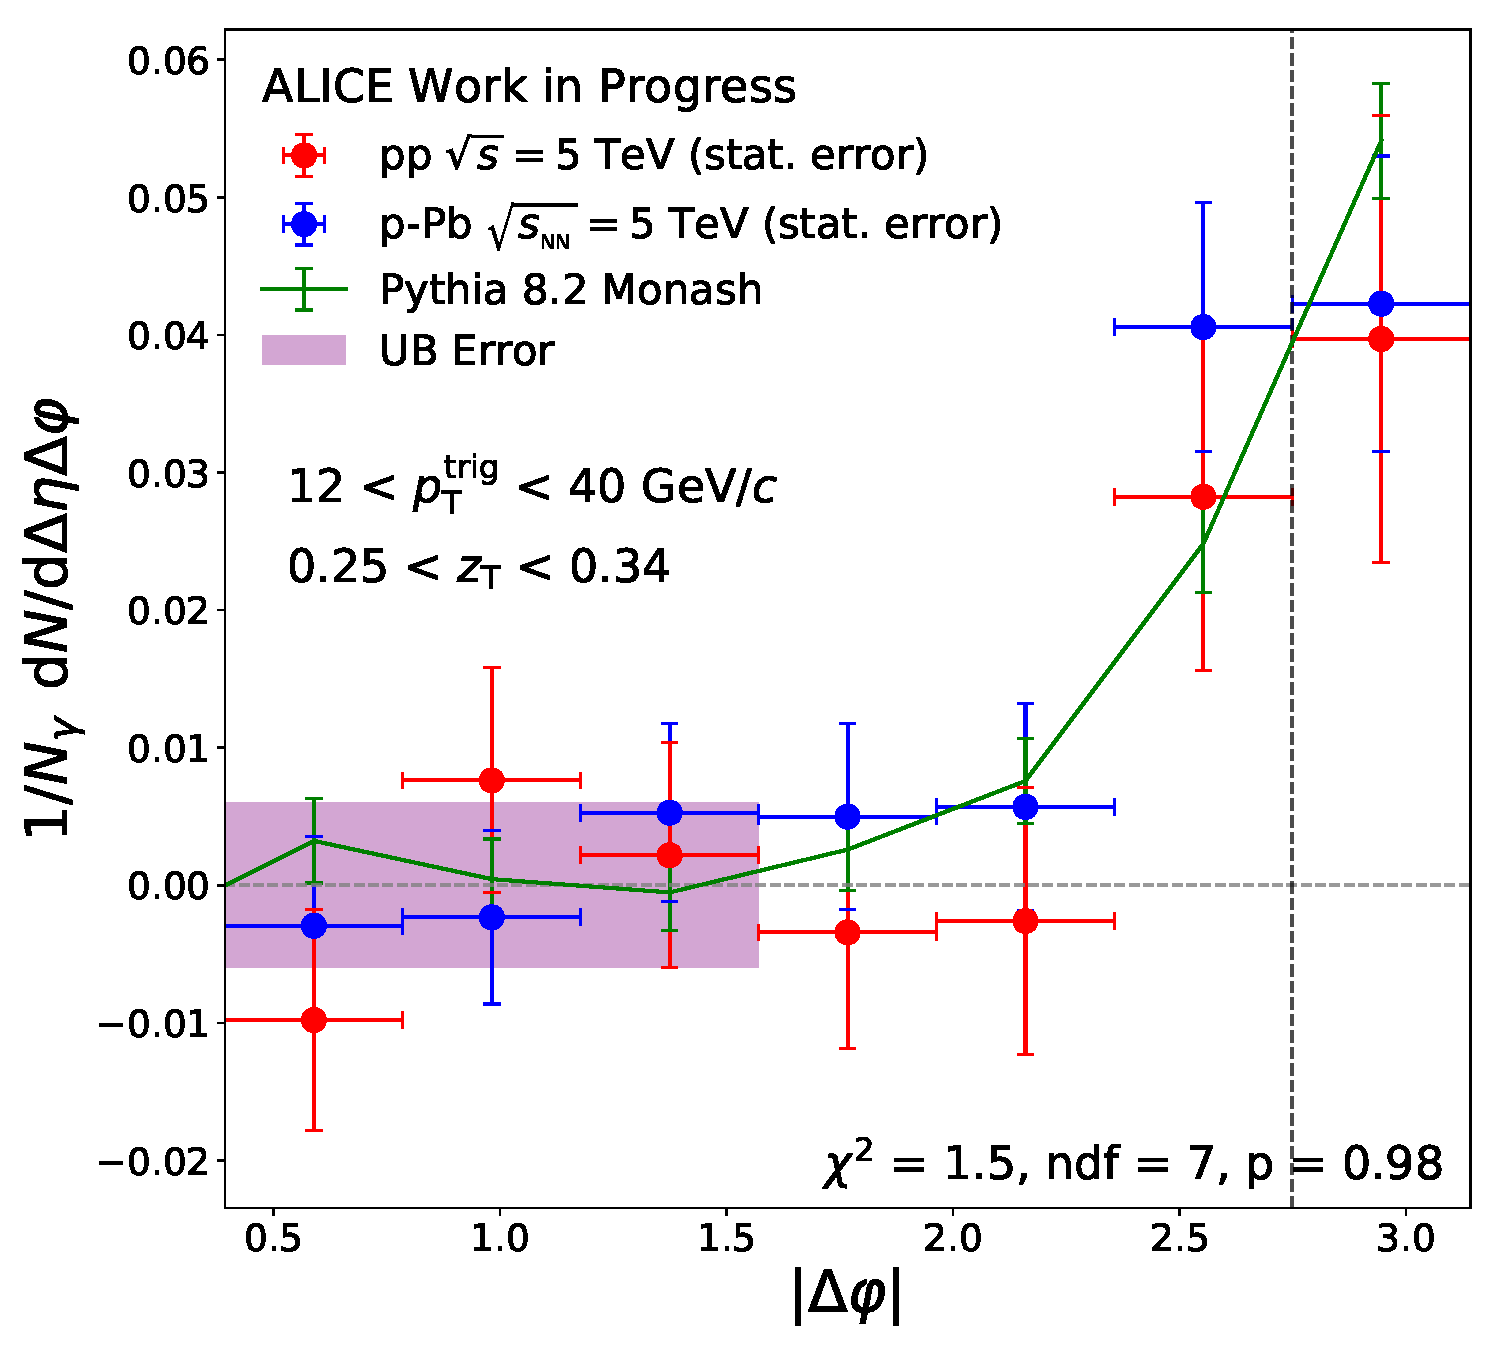
\includegraphics[width = 0.24 \textwidth]{G-H_New/Cs_Final_Indv_pT_0_zT_5.pdf}
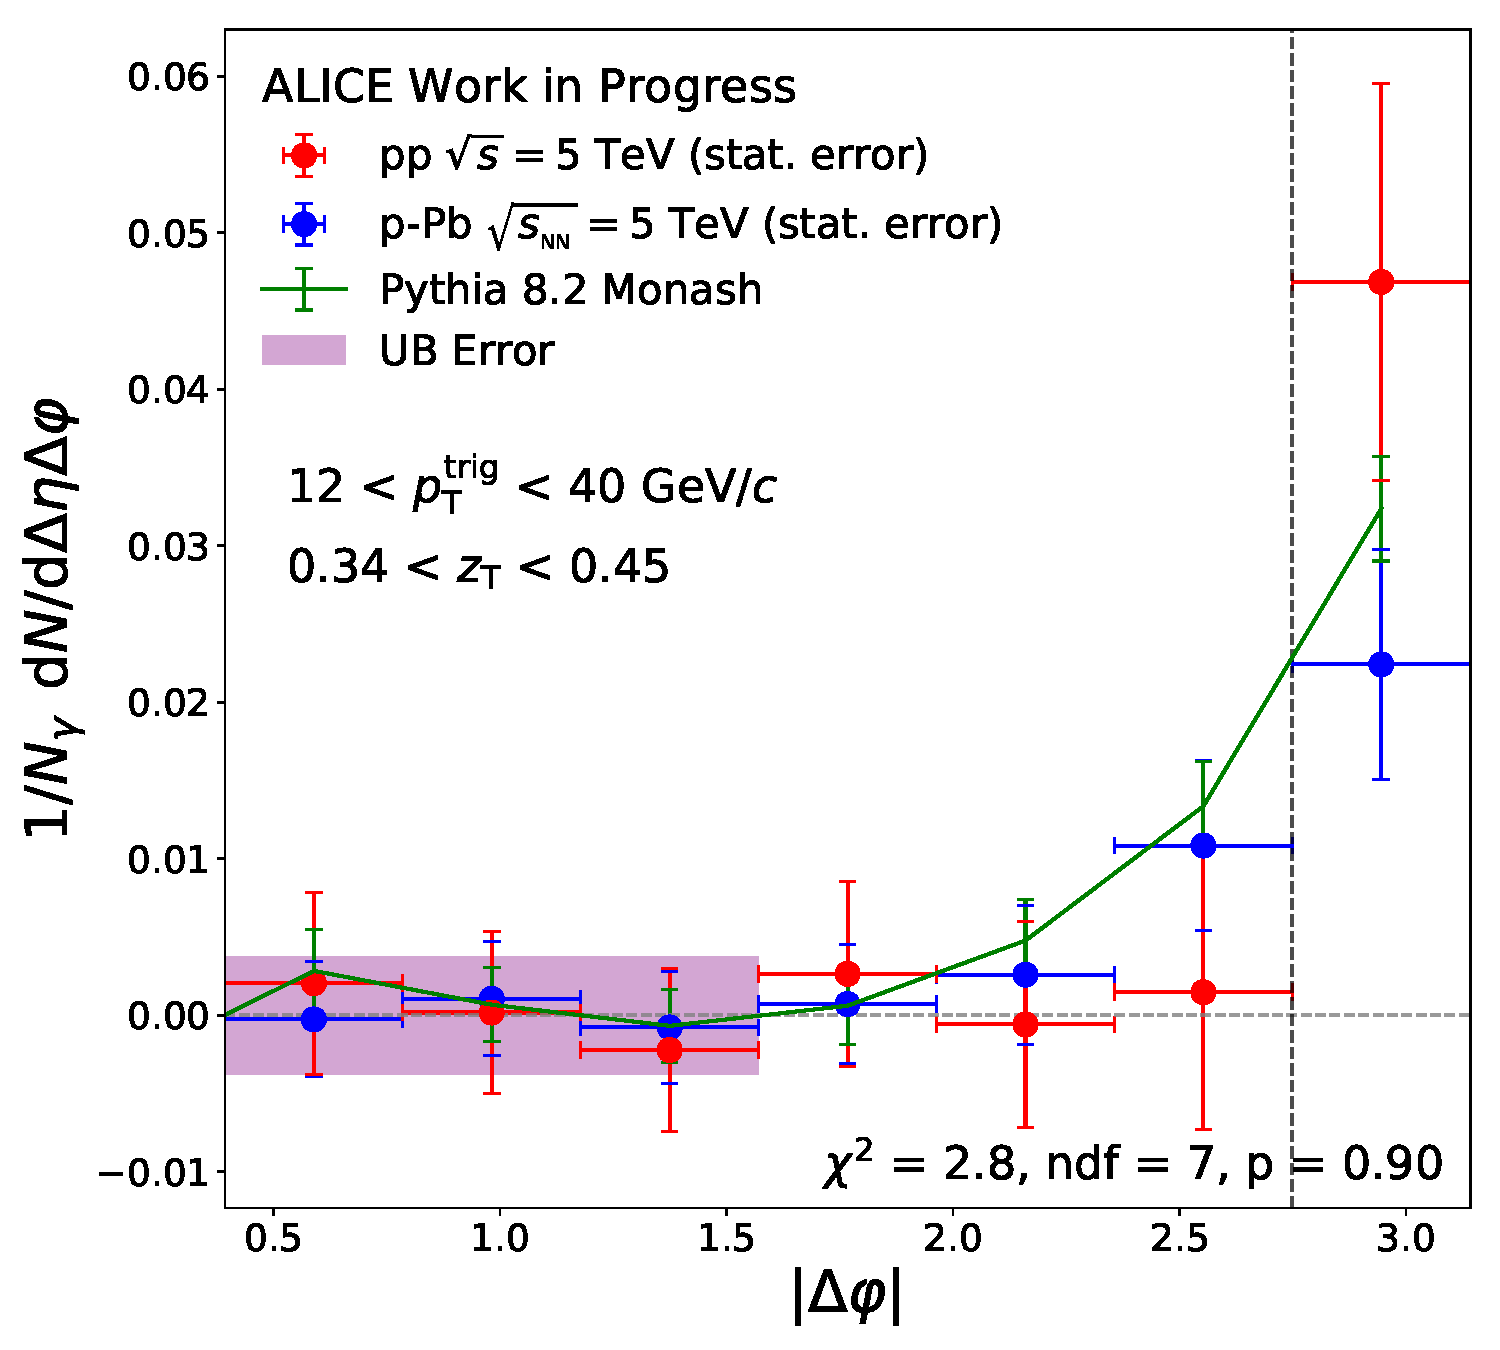
\includegraphics[width = 0.24 \textwidth]{G-H_New/Cs_Final_Indv_pT_0_zT_6.pdf}
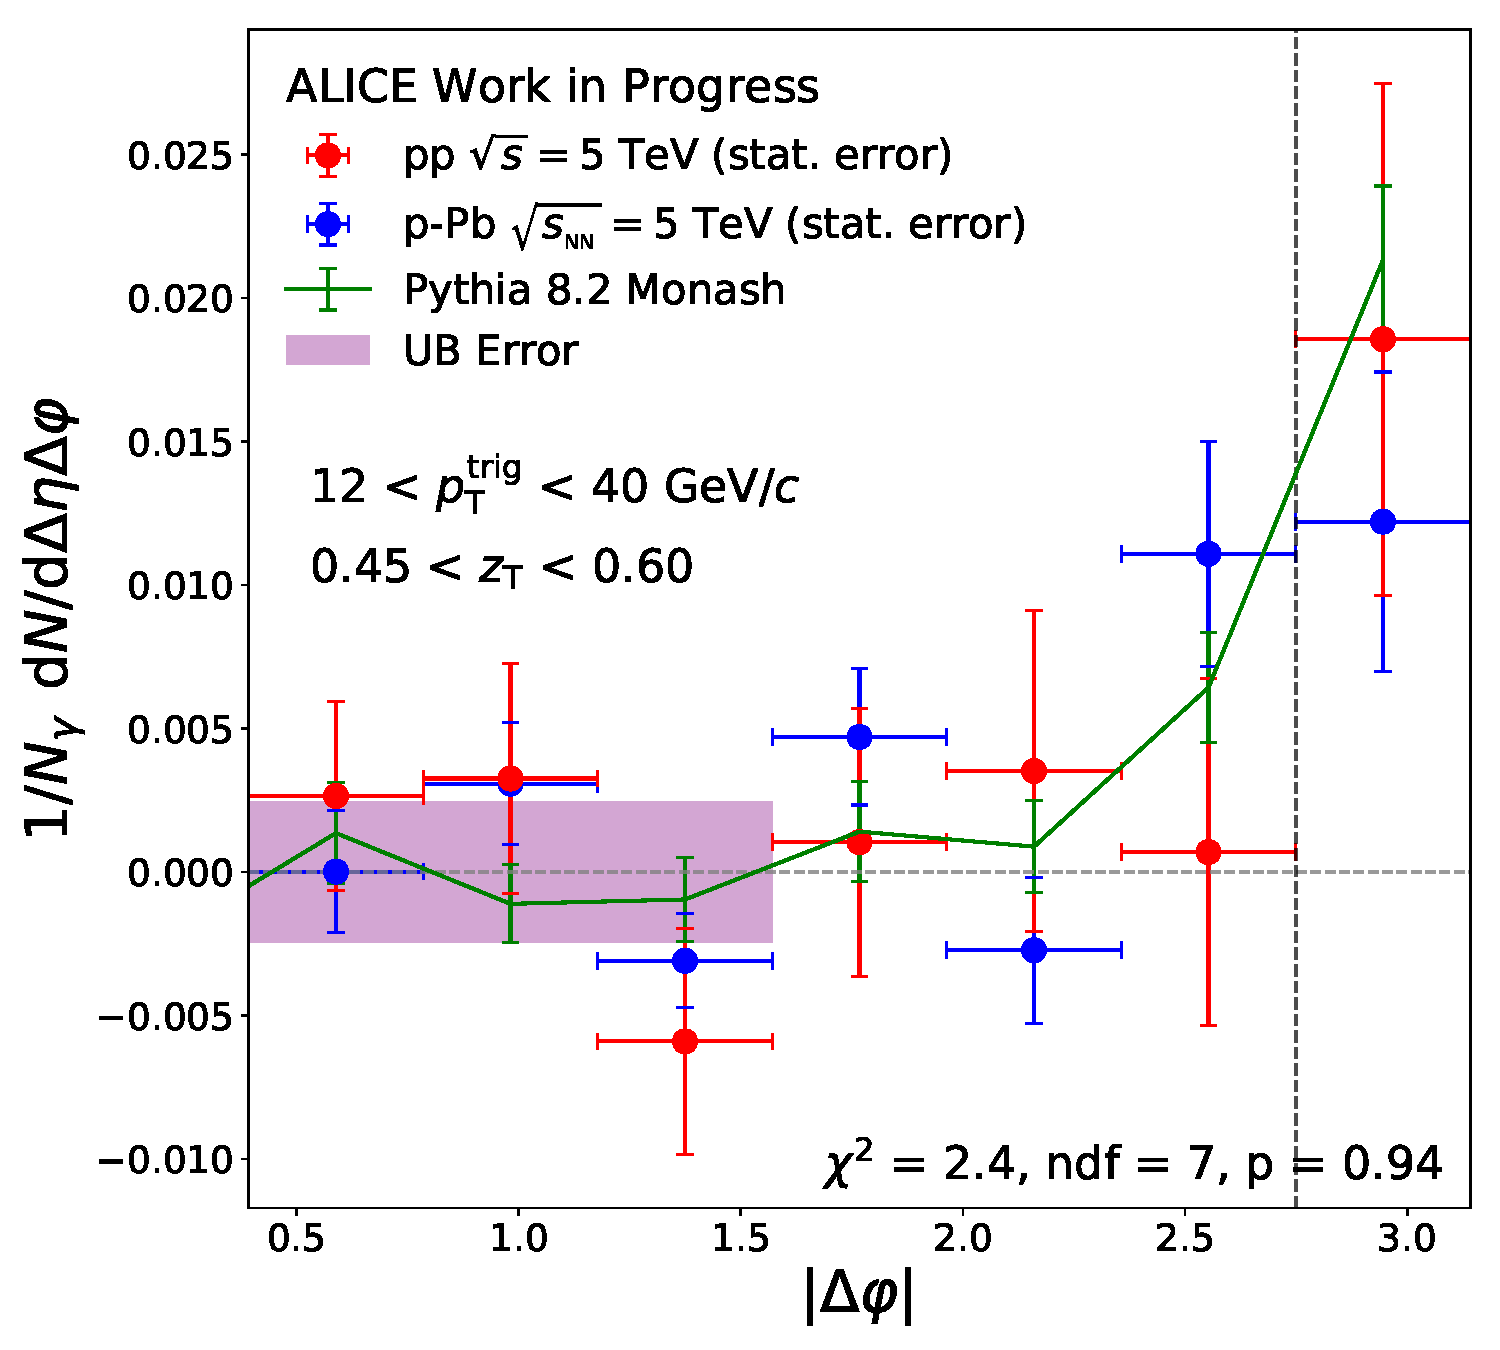
\includegraphics[width = 0.24 \textwidth]{G-H_New/Cs_Final_Indv_pT_0_zT_7.pdf}
\caption{Fully-corrected $\gammaiso$--hadron correlation function pp (red) and \pPb~(blue) data. The purple band represents the uncertainty from the underlying event estimate in pp and \pPb. The error bars represent statistical uncertainty only. The green line is the \gammaiso--hadron correlation function obtained with \textsc{PYTHIA 8.2}.}
\label{fig:CorrelationFinal}
\end{sidewaysfigure}

\subsection{Fragmentation functions in pp \& \pPb~data}
\label{sec:Frag_Function}
Finally, we integrate the \gammaiso--hadron correlation functions in the range $|\Delta\varphi|>7\pi/8$ to roughly correspond to a cone with radius $R=$0.4 used in various jet studies. The integrals are presented as a function of \zt~in Figure~\ref{ff} and Table~\ref{tab:ff}. 

\begin{figure}[h]
\center
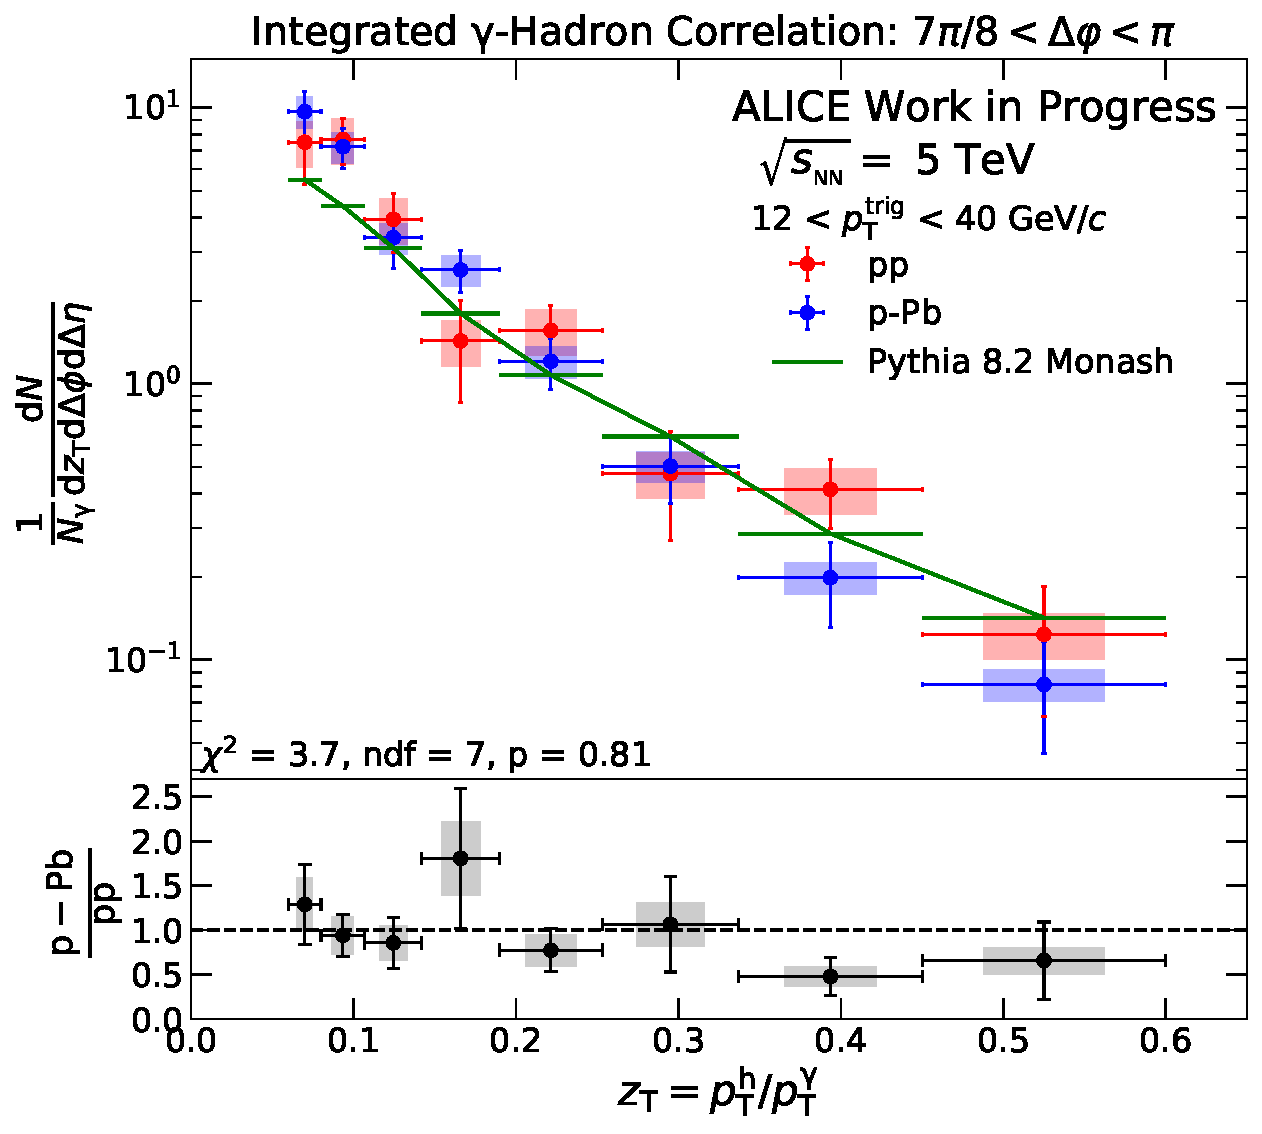
\includegraphics[width=0.8\textwidth]{G-H_New/Final_FFunction_and_Ratio.pdf}
\caption{$\gammaiso$-tagged fragmentation function for pp (red) and \pPb~data (blue). The shaded boxes represent the systematic uncertainties. The green line again represents the \textsc{PYTHIA 8.2} Monash. The $\chi^2$ test for the comparison of pp and \pPb~data incorporates correlations among different \zt~intervals.}
\label{ff}
\end{figure}

\begin{table}
   \centering
   \caption{Summary of uncertainties on integrated away side yields in proton-lead and proton-proton collisions. The uncertainties quoted are absolute.} 
   \begin{tabular*}{1.0\columnwidth}{@{\extracolsep{\fill}}llc@{}}
    \hline
$z_\mathrm{T}$ Range & pp $\pm$ Stat. $\pm$ Sys & p--Pb $\pm$ Stat. $\pm$ Sys. \\
\hline
0.06--0.08 & 7.50$ \pm$ 2.23 $\pm$1.42 & 9.67$ \pm$ 1.82 $\pm$1.27 \\
0.08--0.11 & 7.66$ \pm$ 1.46 $\pm$1.46 & 7.22$ \pm$ 1.18 $\pm$0.94 \\
0.11--0.14 & 3.94$ \pm$ 0.96 $\pm$0.75 & 3.38$ \pm$ 0.76 $\pm$0.44 \\
0.14--0.19 & 1.43$ \pm$ 0.57 $\pm$0.27 & 2.58$ \pm$ 0.44 $\pm$0.34 \\
0.19--0.25 & 1.56$ \pm$ 0.36 $\pm$0.30 & 1.21$ \pm$ 0.25 $\pm$0.16 \\
0.25--0.34 & 0.47$ \pm$ 0.20 $\pm$0.09 & 0.50$ \pm$ 0.14 $\pm$0.07 \\
0.34--0.45 & 0.41$ \pm$ 0.12 $\pm$0.08 & 0.20$ \pm$ 0.07 $\pm$0.03 \\
0.45--0.60 & 0.12$ \pm$ 0.06 $\pm$0.02 & 0.08$ \pm$ 0.04 $\pm$0.01 \\
  \end{tabular*}
   \label{tab:FF_Summary}
\end{table}


\begin{table}[h]
   \centering
   \caption{Number of $\gammaiso$--hadron pairs per $\gammaiso$ integrated in $\Delta\varphi>7\pi/8$, for different $\zt$ intervals. The uncertainty quoted is statistical only. } 
   \begin{tabular*}{1.0\columnwidth}{@{\extracolsep{\fill}}lccc@{}}
    \hline
$\zt$ range & pp & \pPb & \pPb/pp \\
\hline
0.06 - 0.08 & 7.496 $\pm$ 2.230 & 9.666 $\pm$ 1.818 & 1.290 $\pm$ 0.454 \\
0.08 - 0.11 & 7.663 $\pm$ 1.457 & 7.216 $\pm$ 1.182 & 0.942 $\pm$ 0.236 \\
0.11 - 0.14 & 3.943 $\pm$ 0.959 & 3.379 $\pm$ 0.765 & 0.857 $\pm$ 0.285 \\
0.14 - 0.19 & 1.429 $\pm$ 0.571 & 2.584 $\pm$ 0.443 & 1.809 $\pm$ 0.786 \\
0.19 - 0.25 & 1.559 $\pm$ 0.356 & 1.207 $\pm$ 0.253 & 0.774 $\pm$ 0.240 \\
0.25 - 0.34 & 0.473 $\pm$ 0.201 & 0.503 $\pm$ 0.135 & 1.065 $\pm$ 0.536 \\
0.34 - 0.45 & 0.415 $\pm$ 0.116 & 0.198 $\pm$ 0.068 & 0.478 $\pm$ 0.211 \\
0.45 - 0.60 & 0.124 $\pm$ 0.061 & 0.081 $\pm$ 0.036 & 0.658 $\pm$ 0.434 \\
	
\hline 
   \end{tabular*}
   \label{tab:ff}
\end{table}

Figure~\ref{ffRatio} shows the ratio of \pPb~to pp data. The systematic uncertainties in the ratio are described in Section~\ref{sec:systematics}. The uncertainty due to UE-subtraction is fully uncorrelated with $\zt$ and is combined in quadrature with the statistical uncertainty and shown as bars. All other uncertainties are correlated with $\zt$ and shown in boxes. 

\begin{figure}[h]
\center
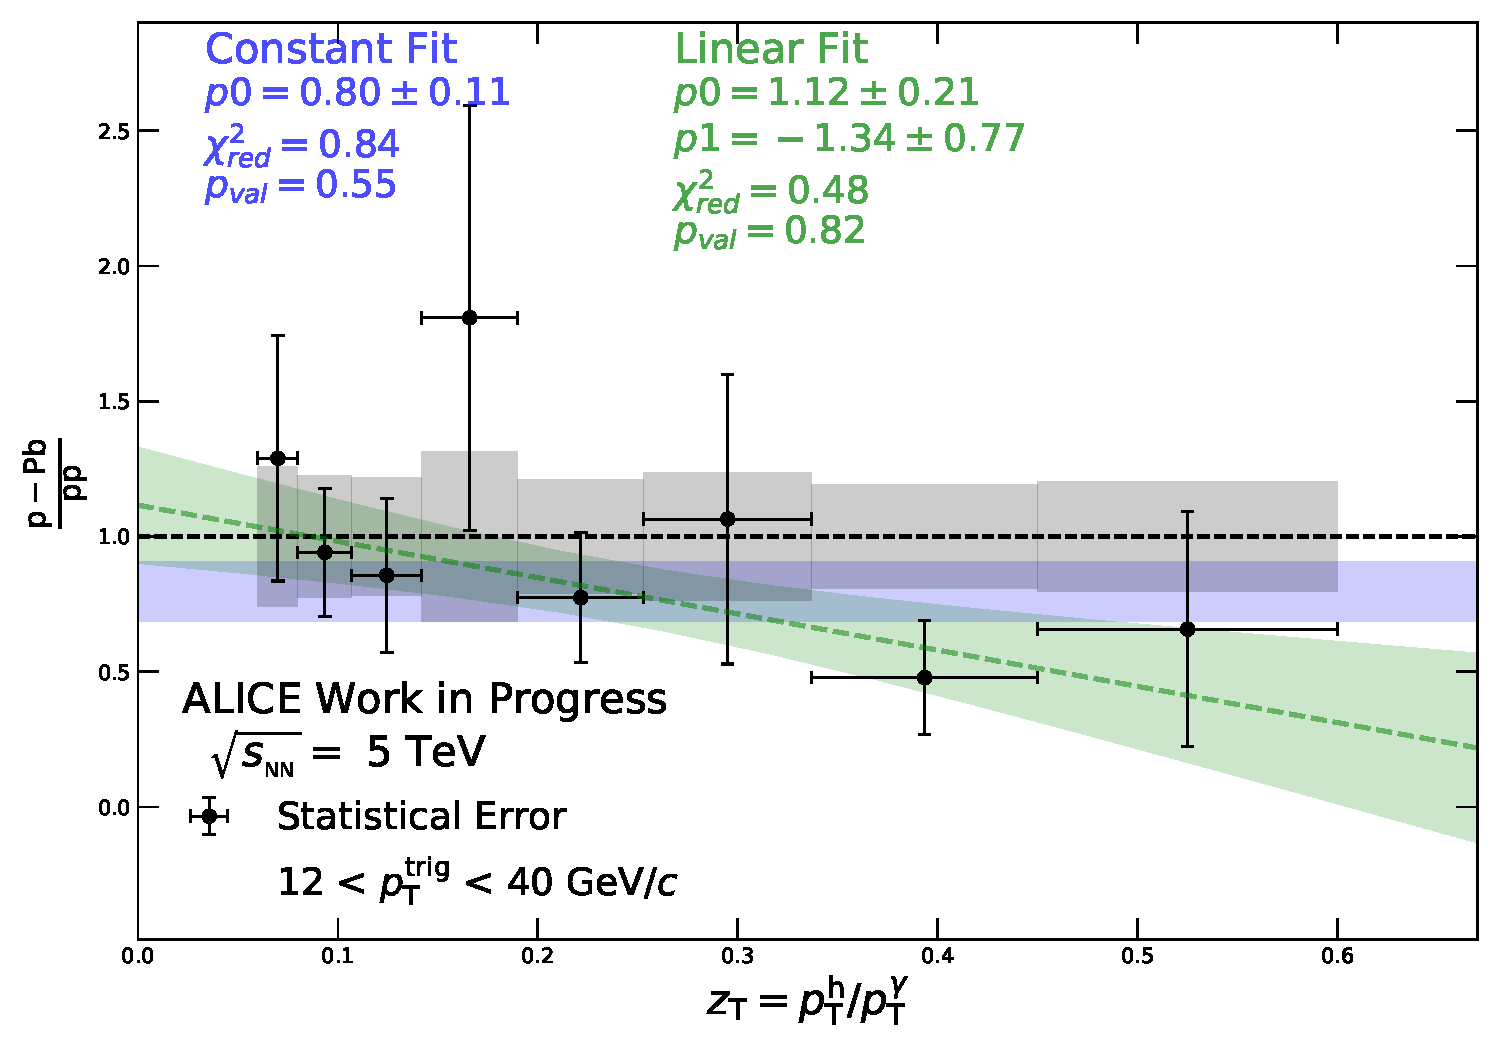
\includegraphics[width=0.6\textwidth]{G-H_New/Ratio_Fits.pdf}
\caption{Ratio of the $\gammaiso$-tagged fragmentation function of \pPb~to pp data. The vertical bars represent statistical uncertainties, and the grey boxes centered at unity represent systematic uncertainties. The horizontal blue band along the the plot represents a constant fit to the ratio. The green line represents a linear fit to the ratio. The widths of both fits represent the 68\% confidence intervals.}
\label{ffRatio}
\end{figure}

The ratio is consistent with unity within uncertainties. We fit the ratio with a constant (using only the uncertainty that is uncorrelated with \zt) and obtain $0.85\pm0.12$ with a reduced $\chi^{2}$ of 0.72. Thus, we find no significant difference between pp and \pPb~$\gammaiso$-tagged fragmentation pattern